\section{Experimental Setup}
Query expansion using pseudo relevance turns out to yield better results in terms of relevance compared to a TF/IDF search,
which is a common approach in todays search engines.
However, to use techniques like query expansion,
the implementation most be fast enough in an interactive environment.
In other words, the results have to be available within 100 ms.
Evaluating both implementations,
will use a multi term search which utilizes TF/IDF.
This search will be used as a baseline to compare the query expansion implementation agins.
Query expansion requires the search engine to process a initial query,
to then later send a new query to retrieve the final result.
As the search requires two searches,
the query expansion implementation will naturally yield higher response times.
The most interesting results are how much slower the query expansion is compared to the baseline search.

\subsection{Data Set}
\label{sec:dataset}
The data set consits of photo data gathered from the Flickr API\footnote{\url{https://www.flickr.com/services/api/}}.
[?? why was Flickr chosen?]
All the photos were retrieved using Flickr's endpoint for fetching the last published photos.
However, the API limits the number of requests per hour.
The photos were gathered over a period of about three months, march 2017 to the end of may 2017.
The data set used in the experiment consists of 4,561,816 photos and 9,993,411 tags.
Of all the photos, a total of 1,708,324 photos have 1 or more tags.
Which means that 37 \% of the photos have tags.
Counting all the photos with at least one tag,
each photo have 5.8 tags on average.
Every tag is user created by the person who posted the photo.
Flickr also have an analyzer which ads addition tags,
but these tags are not available through the API.

The pie chart in figure \ref{fig:pie-chart-tag-distribution} shows the number of tags on each photo.
The pie chart shows that most of the photos have 5 tags.
[?? write more here]

\begin{figure}[h!]
  \centering 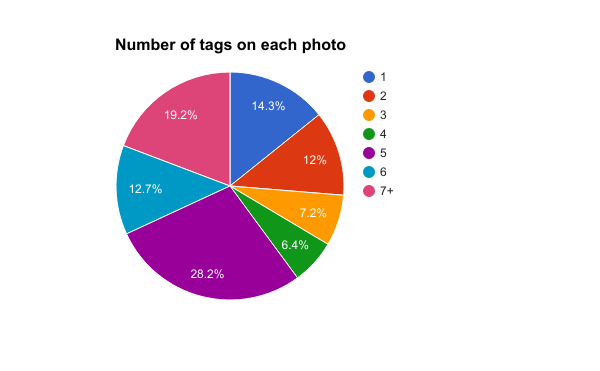
\includegraphics[width=1\linewidth]{img/number-of-tags-distribution.png}
  \caption{Pie chart that shows the distribution on how many tags each photo have.}
  \label{fig:pie-chart-tag-distribution}
\end{figure}

\subsection{Lucene Experiment}
The Lucene experiments starts to build the index with all the photo data.
To make the experiment simpler only the fields: tags, title and url are stored.

\subsection{Elasticsearch Experiment}
The Elasticsearch experimental setup contains two main components, a web server and a search engine.
The web server is implemented in NodeJS and the search engine used is Elasticsearch.

As large applications ofter use cloud providers, the tests also needed to be conducted using cloud providers.
The requirement set for the cloud provider was: need to be videly used, have servers in Europe and provide VPS services.
Possible providers were: Amozon Web Services\footnote{\url{https://aws.amazon.com/}},
Google Cloud Platform\footnote{\url{https://cloud.google.com/}} and Digital Ocean\footnote{\url{https://www.digitalocean.com/}}.
Google Cloud Platform were chosen as the service provider, as you have more flexibility to choose between number of cores and the memory size,
the author had both knowledge to the platform and they gave away free credits[?? Maybe give a better reason?].
Tests were conducted using two Google Compute Engine instances.
Web services always strives to place the servers as close to the users as possible.
To make the experiment simulate a real world scenario both the instances were placed in the reagion called \textit{europe-west1-c}.

\subsubsection{Elasticsearch Instance}
The instance running Elasticsearch had the following specifications: 2 vCPUs, 10 GB memory and 20 GB SSD.
Elasticsearch's documentation\footnote{\url{https://www.elastic.co/guide/en/elasticsearch/guide/current/hardware.html}}
suggest that memory will be the most important resource in most use cases.
As a result more memory were chosen over the number of CPUs.
An important setting in Elasticsearch is the heap size.
By default the heap memory size is set to 1 GB, but were changed to 5 GB in the test environment.
A logical asumption would be to set the Elasticsearch to use all the available memory, except the memory needed for the operating system.
However, Elasticsearch's underlying structure Lucene also needs memory.
Lucene stores the data in separate files.
The datastructure inside the files are immutable, which makes them optimized for caching.
With this strategy Lucene optimizes the underlying operating system's eager to hold small and often used files in memory.
According to the Elasticsearch documentation\footnote{\url{https://www.elastic.co/guide/en/elasticsearch/guide/current/heap-sizing.html}}
the heap size should be set to 50\% or less, of the available memory.

Most operating systems today also comes with swapping turned on by default.
If the operating system decides to swap it would significantly reduce the performance.
To avoid the problem swapping were turned off on the Elasticsearch instance.

\subsubsection{NodeJS Instance}
The instance running NodeJS had the following specifications: 4 vCPUs, 4 GB memory and 10 GB SSD.
On the web server we want to be able to handle as many requests as possible.
The number of requests the server is able to handle are closely linked to the number of cores.
That is why the Node.js instance has more cores at the cost of less memory.

Node.js is by design single threaded, which would make 3 of the cores on the Node.js server being idle.
However, this problem can be solved by using tool called pm2\footnote{\url{http://pm2.keymetrics.io/}}.
pm2 has a feature called \textit{cluster mode}, which may spawn multple Node.js instances.
To allow maximum CPU utilization, pm2 can be configured to spawn as many Node.js instances as the number of cores.

To test the implementation the Node.js web server implemented two different endpoints.

- Node.js, version
- Configuration NODE\_ENV=production
- pm2
- two endpoints, one for base line one for query expansion



\subsection{Performance Metrics}
Evaluating the implementation is done by measuring the response time from a client sends the request to the response arrives.


\begin{figure}[h!]
  \centering 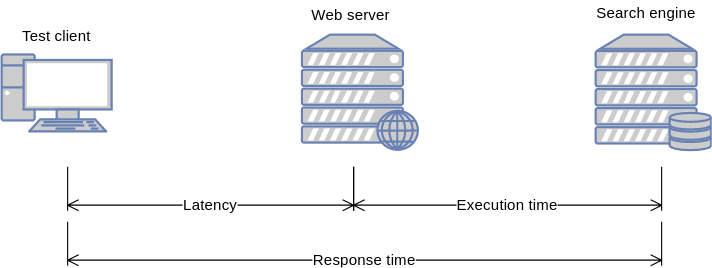
\includegraphics[width=0.9\linewidth]{img/latency-measurements.png}
  \caption{Overview of the different measurements used when evaluating the implementation.}
  \label{fig:latency-measurements}
\end{figure}
